\section{Chip configuration and programming}

The toolchain used for configuring and programming the chip consists of STM32CubeMX\footnote{https://www.st.com/en/development-tools/stm32cubemx.html} and the free version of Keil µVision\footnote{http://www2.keil.com/mdk5/uvision/}.

\subsection{Configuration}

STM32CubeMX software provides a simple, yet powerful interface for the configuration of MCUs. After selecting the board, user is able to set each pins purpose.

\subsection{Clock}
There are four options to be used for the measurement of the system tick: HSI\footnote{HSI - High Speed Internal}, HSE\footnote{HSE - High Speed External}, LSI\footnote{LSI - Low Speed Internal}, LSE\footnote{LSE - Low Speed Exteral}. Even though a HSI has a less accurate tick, it was used in this project due to its faster startup time compared to HSE. The frequency of the clock is set to 8Mhz on APB1 output which is used by both timers and peripheral clocks. 


\begin{figure}[htbp]
    \centerline{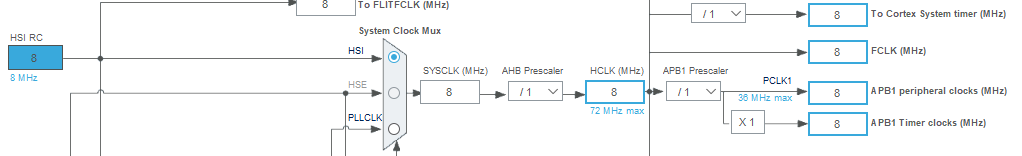
\includegraphics[width=9cm]{Images/Clock.png}}
    \caption{Clock configuration}
    \label{fig7}
\end{figure}

\subsection{Timers}
The chip offers four timers with four channels each which can be used for system interrupts and pulse width modulation. 
In this setup TIM1s first channel was used to produce a timed interrupt every second when the process of obstacle detection happens. 
The second utilized timer TIM2s second channel was used to generate a pwm on the pin A1.

\subsection{Pinout}
Fourteen pins were configured of which eleven are used as either GPIO input or output pins, two are used for UART communication and one is a pulse width modulation pin

\begin{figure}[htbp]
    \centerline{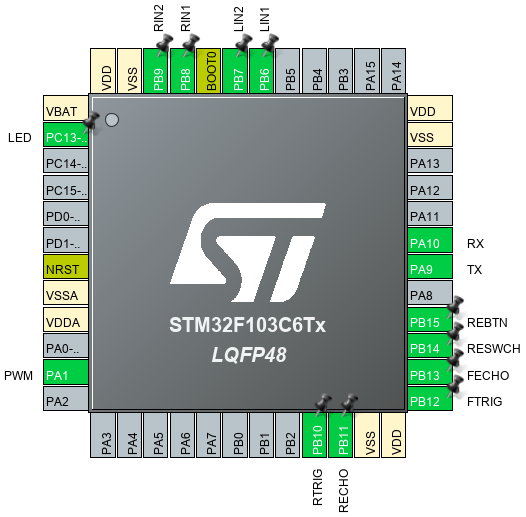
\includegraphics[width=9cm]{Images/Pinout.png}}
    \caption{Pinout}
    \label{fig8}
\end{figure}

\subsection{Source code}
The source code was written and compiled in Keil µVision. Embedded-C is the most popular choice for programming the HAL\footnote{Hardware Abstraction Layer}. There was a small library of functions and structures created for handling the motors and the movement of the rover as well as setting up and acquiring data from the ultrasonic sensors. The full source code can be found on the projects GitHub page\footnote{https://www.github.com/Adi-Sose/Rover}. For the purpose of keeping this paper short the functions purposes will be explained with no code inserted.
\begin{itemize}
    \item Motor set is a structure which holds the information about the two pins a motor uses.
    \begin{itemize}
        \item Setup function initializes the object with the passed values.
        \item Set direction function sets the pins in such a state that the motors run in chosen direction.
        \item Stop function sets the pins states in such a combination that the motor stops moving.
    \end{itemize}
    \item Motion controller is a project specific structure holding the information about two motorsets - the left and the right set of motors. It also provides information about current rotation or direction of the rover and allows for a blocking mechanism of movement direction.
    \begin{itemize}
        \item Setup function initializes the object with the passed values.
        \item Set direction sets both motor sets in a state which allows the rover to move in a chosen direction.
        \item Set rotation sets both motor sets in a state which allows the rover to rotate in a chosen direction.
        \item Stop function sends the stopping signal to both motorsets
        \item Block direction disables the movement direction for the rover and acts as a locking mechanism to prevent movement in specified direction.
        \item Unblock direction allows the rover to move in that direction once again.
    \end{itemize}
    \item Ultrasonic structure holds the information about the TRIG and ECHO pin of a sensor
    \begin{itemize}
        \item Setup function initializes the object with the passed values.
        \item Get distance function sends a 10ms signal to the TRIG pin and waits for the ECHO pin to send its signal. After this step the program gets the time before and after the ECHO ping was set to its high state and performs a calculation to return the distance of the nearest object to the sensor.
    \end{itemize}
\end{itemize}

While the rover is in its idle state, the controller is waiting for the input on its UART pin. Based on the signal that was passed by the Android phone with the app installed it determines in which direction the user wants the rover to move in. The movement stop once the user sends a stop signal or when the external interrupt which has the task to measure distance of the rover from obstales sends the blocking command to the motion controller. The purpose of encoder is to control the speed of the rover, by turning the knob an interrupt is triggered which then updates the duty cycle of pwm based on the direction of the rotation. 